\hypertarget{ux438ux43dux444ux43eux440ux43cux430ux446ux438ux44f}{%
\section{Информация}\label{ux438ux43dux444ux43eux440ux43cux430ux446ux438ux44f}}

\begin{frame}{Докладчик}
\protect\hypertarget{ux434ux43eux43aux43bux430ux434ux447ux438ux43a}{}
\begin{itemize}
\tightlist
\item
  Рыжкова Ульяна Валерьевна
\item
  студент
\item
  Российский университет дружбы народов
\end{itemize}
\end{frame}

\hypertarget{ux437ux430ux434ux430ux43dux438ux435-1.-ux441ux43eux437ux434ux430ux43dux438ux435-ux43dux43eux432ux43eux433ux43e-ux444ux430ux439ux43bux430-ux441-ux438ux441ux43fux43eux43bux44cux437ux43eux432ux430ux43dux438ux435ux43c-vi}{%
\section{Задание 1. Создание нового файла с использованием
vi}\label{ux437ux430ux434ux430ux43dux438ux435-1.-ux441ux43eux437ux434ux430ux43dux438ux435-ux43dux43eux432ux43eux433ux43e-ux444ux430ux439ux43bux430-ux441-ux438ux441ux43fux43eux43bux44cux437ux43eux432ux430ux43dux438ux435ux43c-vi}}

\begin{frame}{Задание 1. Создание нового файла с использованием vi}
\begin{enumerate}
\tightlist
\item
  Создаём каталог и переходим в него
\end{enumerate}

\begin{figure}
\hypertarget{fig:001}{%
\centering
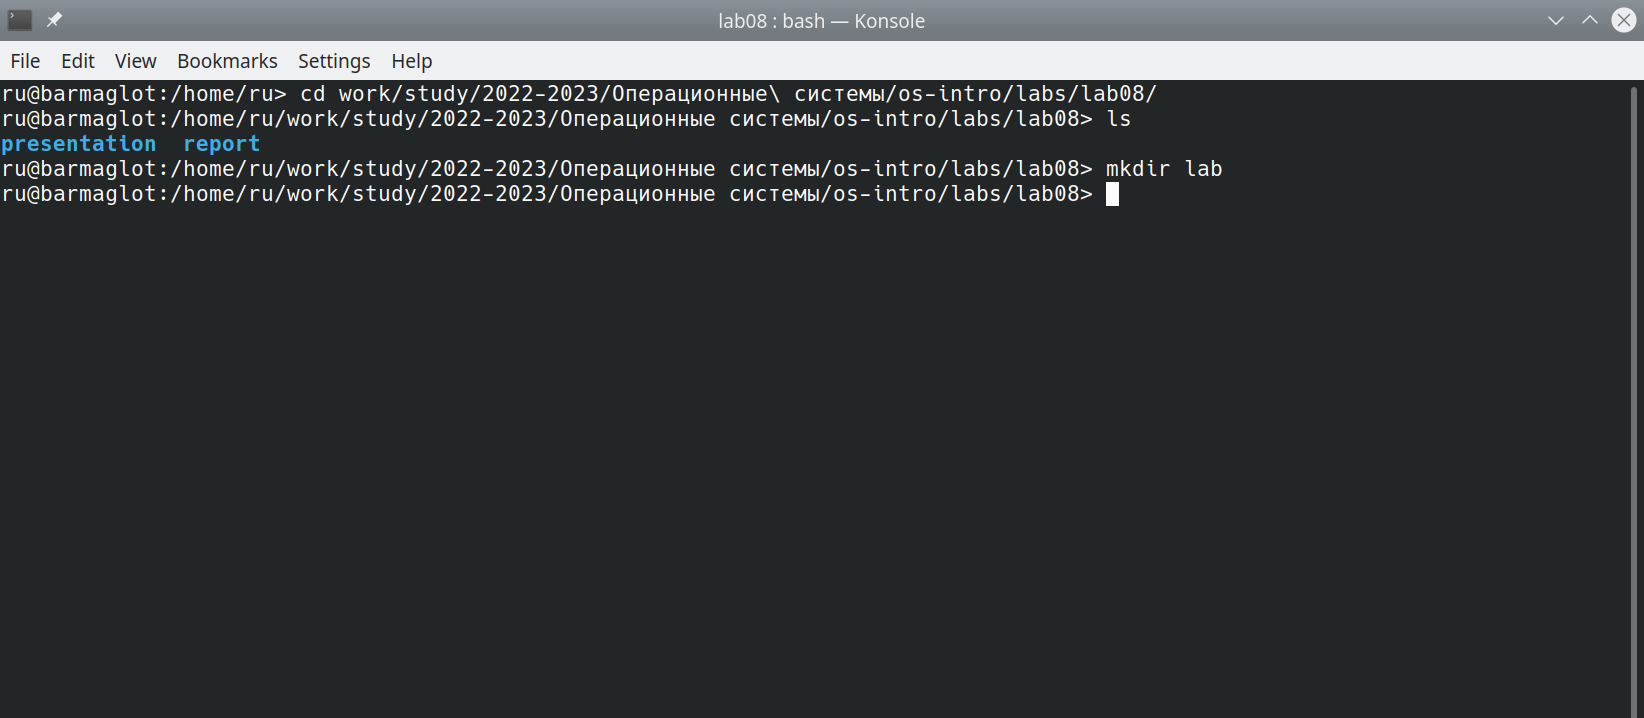
\includegraphics[width=1\textwidth,height=\textheight]{image/1.png}
\caption{Создание каталога}\label{fig:001}
}
\end{figure}

\begin{enumerate}
\setcounter{enumi}{1}
\tightlist
\item
  Создаём файл с помощью команды vi hello.sh
\end{enumerate}

\begin{figure}
\hypertarget{fig:002}{%
\centering
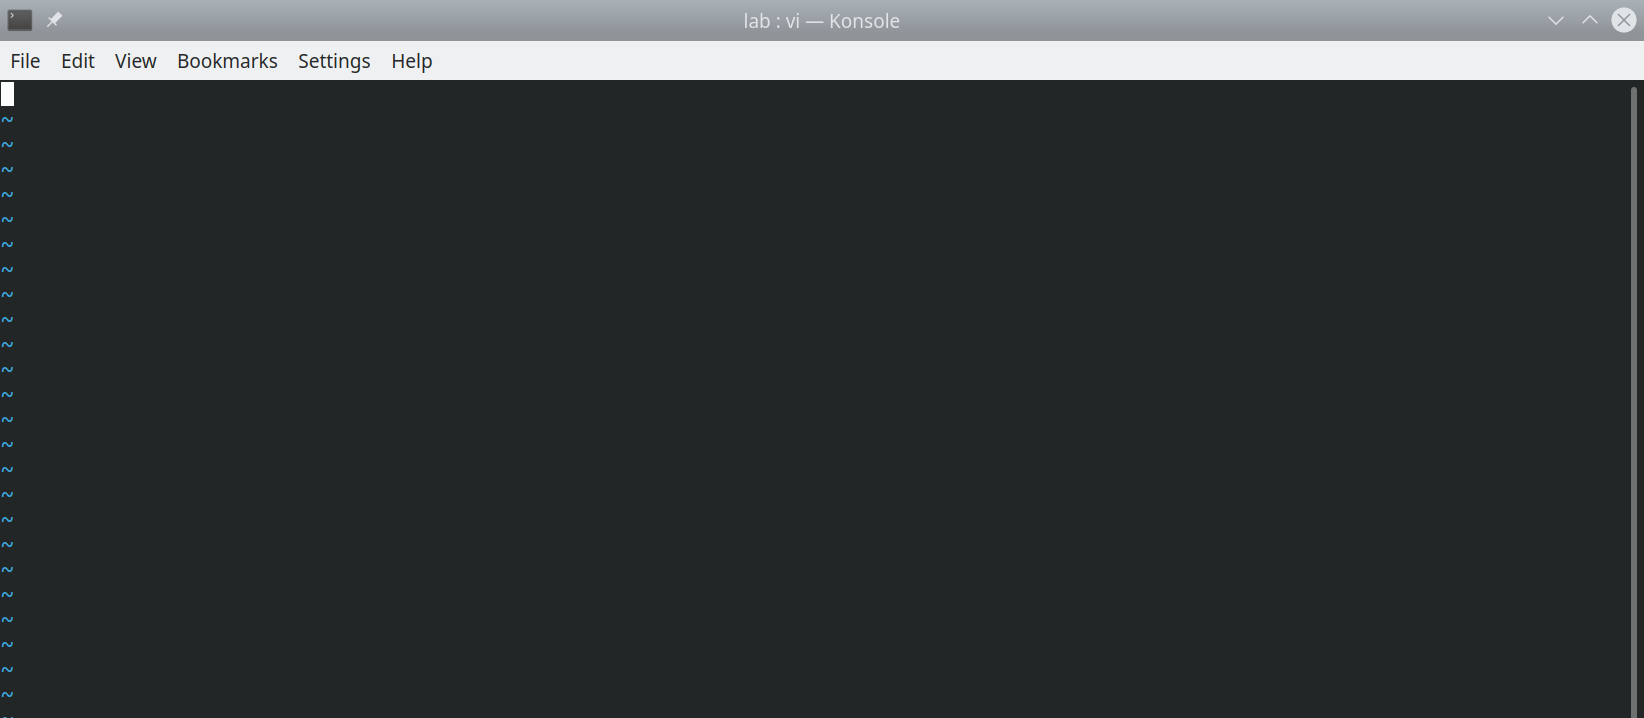
\includegraphics[width=1\textwidth,height=\textheight]{image/2.png}
\caption{Новый файл}\label{fig:002}
}
\end{figure}

\begin{enumerate}
\setcounter{enumi}{2}
\tightlist
\item
  Вводим текст, и с помощью комбинации :wq сохраняем изменения и выходим
  из редактора
\end{enumerate}

\begin{figure}
\hypertarget{fig:003}{%
\centering
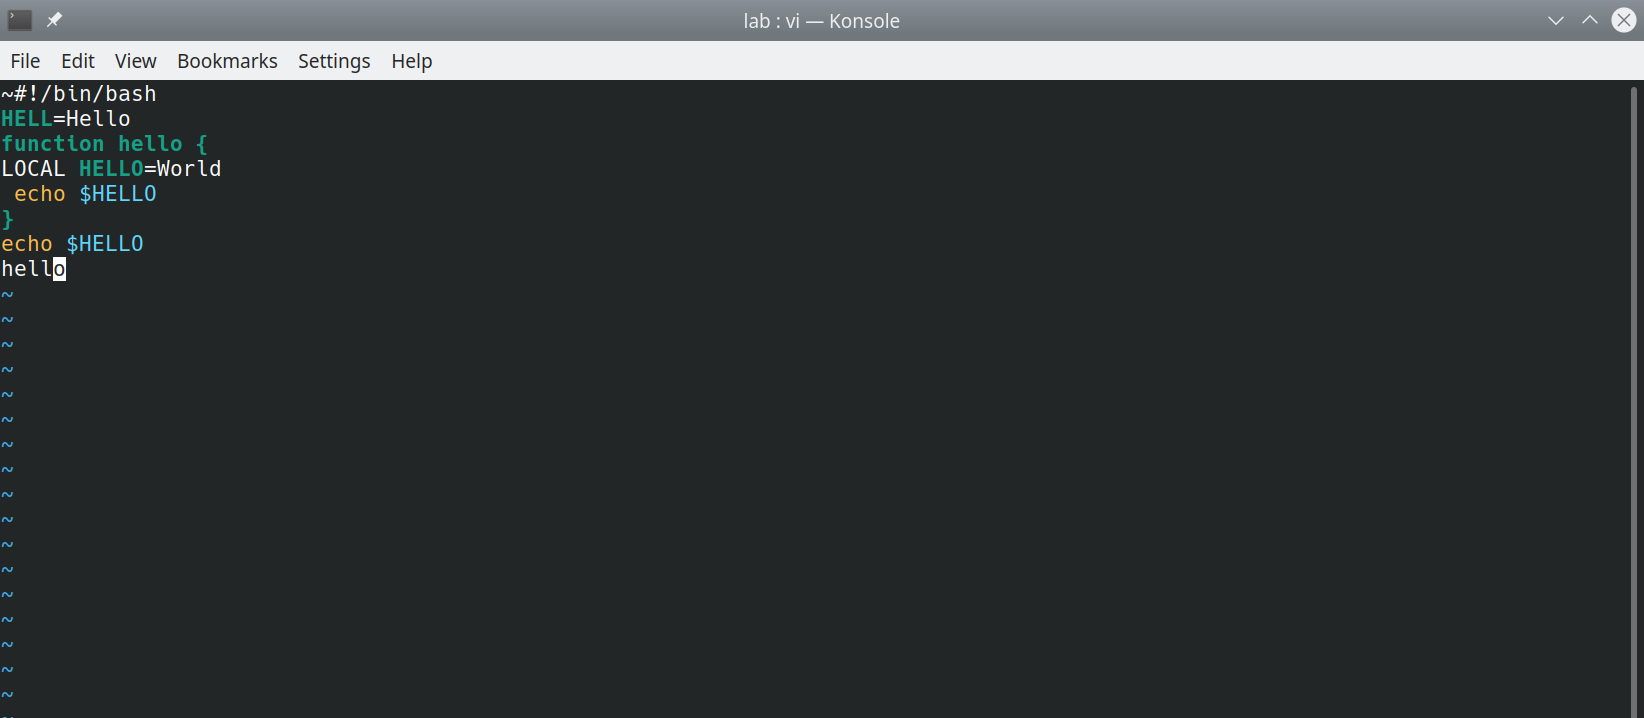
\includegraphics[width=1\textwidth,height=\textheight]{image/4.png}
\caption{Сохранённый текст}\label{fig:003}
}
\end{figure}

\begin{enumerate}
\setcounter{enumi}{3}
\tightlist
\item
  Делаем файл исполняемым
\end{enumerate}

\begin{figure}
\hypertarget{fig:004}{%
\centering
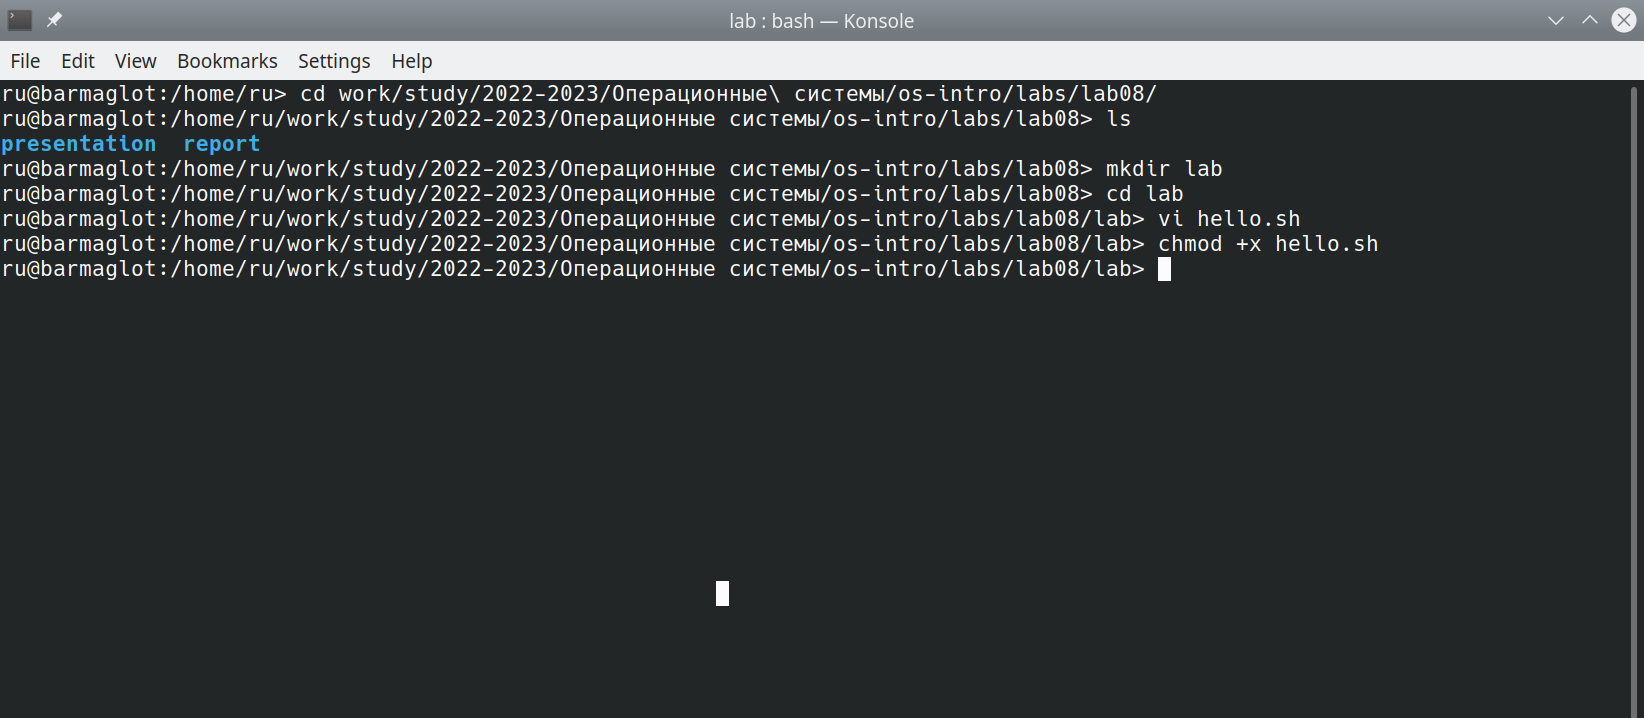
\includegraphics[width=1\textwidth,height=\textheight]{image/3.png}
\caption{Команда chmod +x}\label{fig:004}
}
\end{figure}
\end{frame}

\hypertarget{ux437ux430ux434ux430ux43dux438ux435-2.-ux440ux435ux434ux430ux43aux442ux438ux440ux43eux432ux430ux43dux438ux435-ux441ux443ux449ux435ux441ux442ux432ux443ux44eux449ux435ux433ux43e-ux444ux430ux439ux43bux430}{%
\section{Задание 2. Редактирование существующего
файла}\label{ux437ux430ux434ux430ux43dux438ux435-2.-ux440ux435ux434ux430ux43aux442ux438ux440ux43eux432ux430ux43dux438ux435-ux441ux443ux449ux435ux441ux442ux432ux443ux44eux449ux435ux433ux43e-ux444ux430ux439ux43bux430}}

\begin{frame}{Задание 2. Редактирование существующего файла}
\begin{enumerate}
\item
  Вызвав vi на редактирование файла, устанавливаем курсор в конец слова
  HELL 2-ой строки, используя комбинацию 2G и 5 пробелов
\item
  Переходим в режим вставки, нажав i, добавляем букву O, и, нажав esc,
  возвращаемся в командный режим
\end{enumerate}

\begin{figure}
\hypertarget{fig:005}{%
\centering
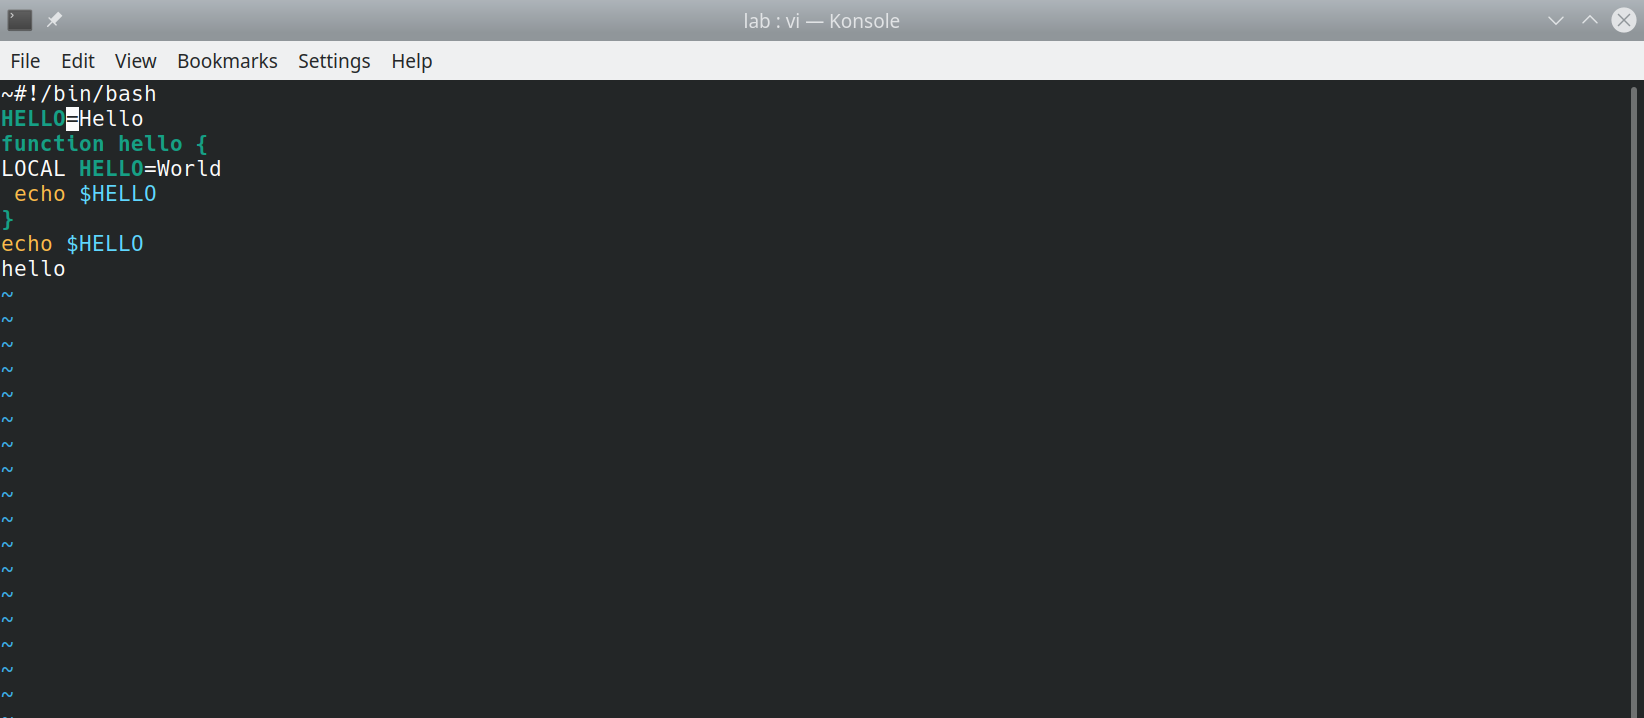
\includegraphics[width=1\textwidth,height=\textheight]{image/5.png}
\caption{Ввели слово HELLO}\label{fig:005}
}
\end{figure}

\begin{enumerate}
\setcounter{enumi}{2}
\tightlist
\item
  Переходим в 4-ую строку (комбинация 4G) и стираем слово LOCAL
  (комбинация dw)
\end{enumerate}

\begin{figure}
\hypertarget{fig:006}{%
\centering
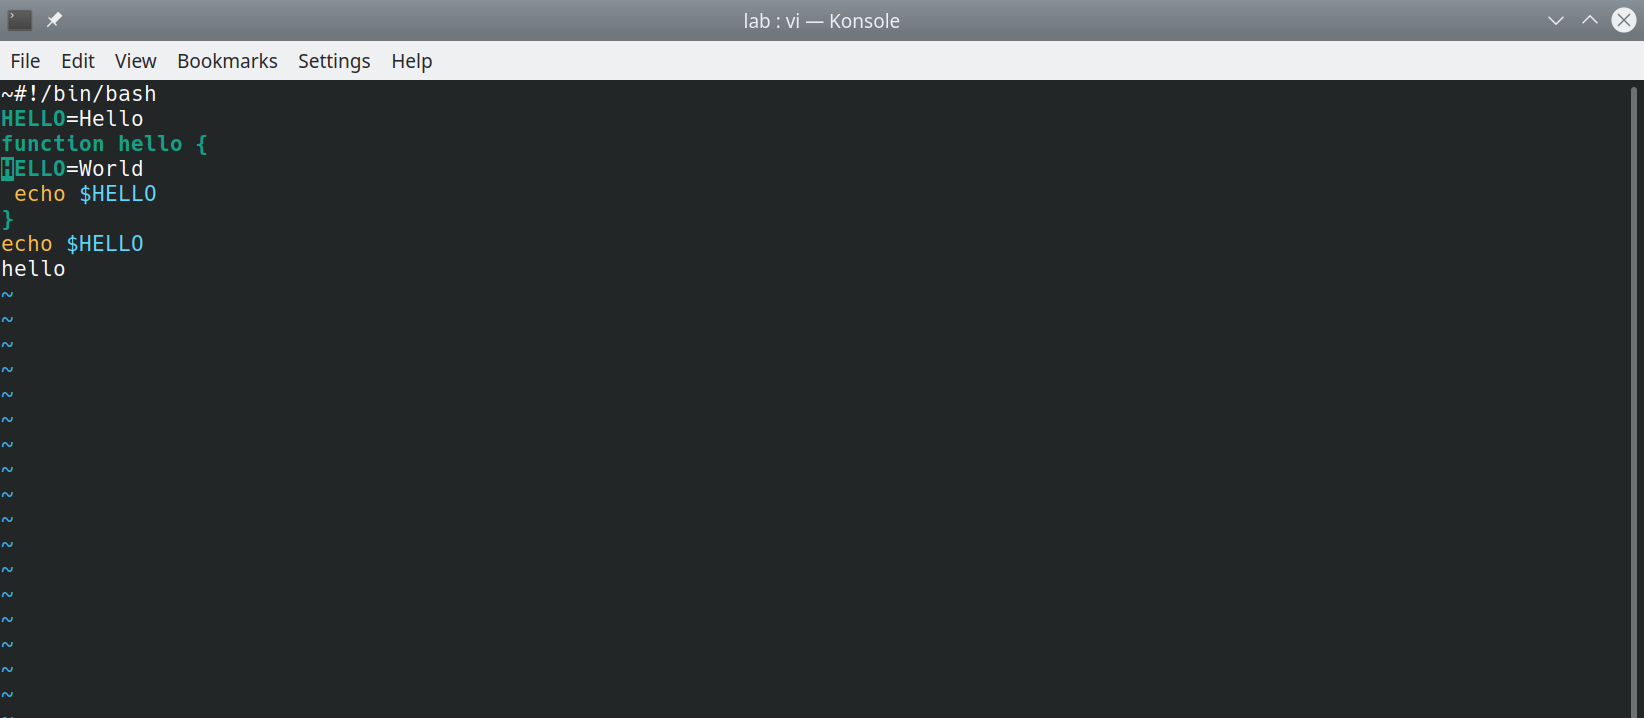
\includegraphics[width=1\textwidth,height=\textheight]{image/6.png}
\caption{Удалили слово LOCAL}\label{fig:006}
}
\end{figure}

\begin{enumerate}
\setcounter{enumi}{3}
\tightlist
\item
  Переходим в режим вставки (i), вводим слово `local', и возвращаемся в
  командный режим (esc)
\end{enumerate}

\begin{figure}
\hypertarget{fig:007}{%
\centering
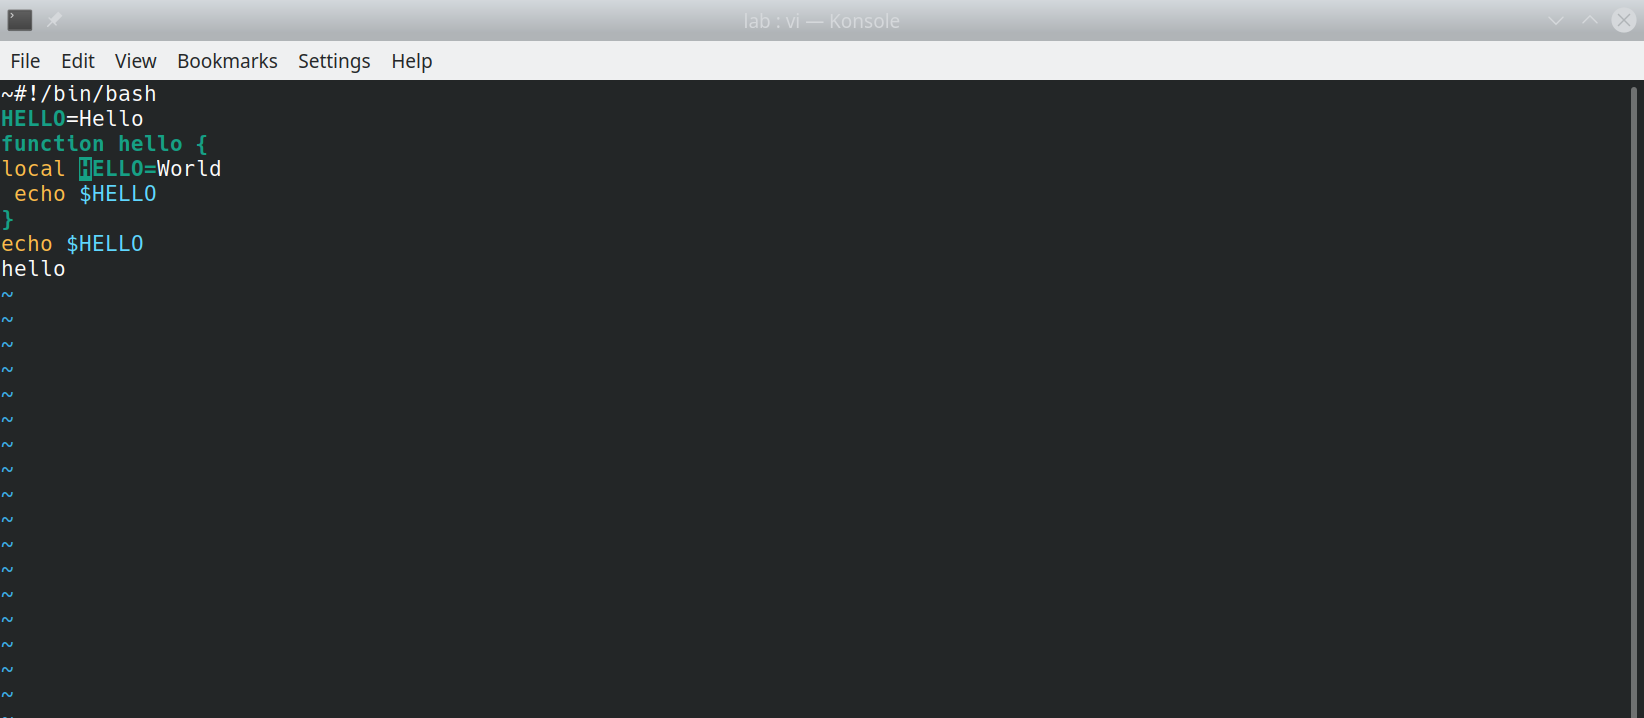
\includegraphics[width=1\textwidth,height=\textheight]{image/7.png}
\caption{Ввели слово local}\label{fig:007}
}
\end{figure}

\begin{enumerate}
\setcounter{enumi}{4}
\item
  Перемещаемся в последнюю строку (G), вставляем пустую строку (о) и
  вводим текст
\item
  Удаляем последнюю строку с помощью комбинации dd. Отменяем последнее
  действие клавишей u
\item
  Вводим :wq, чтобы сохранить изменения и выйти из файла.
\end{enumerate}
\end{frame}
